\documentclass[aspectratio=169,11pt]{beamer}

% ============================ theme & packages ============================
\usetheme{Boadilla}
\usecolortheme{seahorse}
\setbeamertemplate{navigation symbols}{}
\setbeamertemplate{footline}[frame number]
\setbeamertemplate{section in toc}[sections numbered]

\usepackage[T1]{fontenc}
\usepackage[utf8]{inputenc}
\usepackage{lmodern}
\usepackage{amsmath,amssymb,mathtools,bm}
\usepackage{booktabs}
\usepackage{array}
\newcolumntype{L}[1]{>{\raggedright\arraybackslash}p{#1}}
\usepackage{xcolor}
\usepackage{tikz}
\usetikzlibrary{arrows.meta,positioning,shapes.geometric,fit,calc,backgrounds}

% ----- palette -----
\definecolor{cSimplex}{HTML}{2563EB}
\definecolor{cTree}{HTML}{15803D}
\definecolor{cLatent}{HTML}{7C3AED}
\definecolor{cLik}{HTML}{C2410C}
\definecolor{cAccent}{HTML}{BE185D}
\definecolor{cMuted}{HTML}{475569}

\setbeamercolor{block title}{fg=white,bg=cSimplex}
\setbeamercolor{block title alerted}{fg=white,bg=cLik}
\setbeamercolor{block title example}{fg=white,bg=cTree}

% ----- math shortcuts -----
\newcommand{\code}[1]{{\small\texttt{\detokenize{#1}}}}
\newcommand{\R}{\mathbb R}
\newcommand{\N}{\mathbb N}
\newcommand{\KL}{\operatorname{KL}}
\newcommand{\ilr}{\operatorname{ilr}}
\newcommand{\clr}{\operatorname{clr}}
\newcommand{\softmax}{\operatorname{softmax}}
\newcommand{\diag}{\operatorname{diag}}
\newcommand{\Cov}{\operatorname{Cov}}
\newcommand{\E}{\mathbb E}
\newcommand{\Tree}{\mathcal T}
\newcommand{\Inodes}{\mathcal I}
\newcommand{\Ch}{\operatorname{Ch}}
\newcommand{\CE}{\operatorname{CE}}
\newcommand{\Simplex}{\Delta^{p-1}}

% ----- tikz styles -----
\tikzset{
  data/.style ={draw, rounded corners=2pt, align=center, font=\footnotesize,
                minimum height=8mm, inner sep=3pt, fill=cSimplex!12, draw=cSimplex},
  net/.style  ={draw, rounded corners=2pt, align=center, font=\footnotesize,
                minimum height=8mm, inner sep=3pt, fill=cTree!12, draw=cTree},
  lat/.style  ={draw, rounded corners=2pt, align=center, font=\footnotesize,
                minimum height=8mm, inner sep=3pt, fill=cLatent!14, draw=cLatent},
  lik/.style  ={draw, rounded corners=2pt, align=center, font=\footnotesize,
                minimum height=8mm, inner sep=3pt, fill=cLik!14, draw=cLik},
  leaf/.style ={draw, circle, inner sep=1pt, minimum size=5mm, fill=cSimplex!18, draw=cSimplex},
  inode/.style={draw, circle, inner sep=1pt, minimum size=5mm, fill=cTree!18, draw=cTree},
  arrow/.style={-{Latex[length=2mm]}, thick, draw=cMuted},
  darrow/.style={-{Latex[length=2mm]}, thick, dashed, draw=cMuted},
}

% ============================ title ============================
\title[Compositional VAEs in biomevae]{Compositional, tree-aware VAEs in \texttt{biomevae}}
\subtitle{Model diagrams and mathematics: PhILR-VAE, TreeDTM-VAE, CAPDA-VAE}
\author{biomevae}
\date{\today}

\begin{document}

{\setbeamercolor{background canvas}{bg=cSimplex!8}
\begin{frame}[plain]\titlepage\end{frame}}

\begin{frame}{Outline}
  \tableofcontents
\end{frame}

% ====================================================================
\section{Setup: compositional microbiome data}
% ====================================================================
\begin{frame}{The data lives on the simplex}
  \begin{columns}[T]
    \begin{column}{0.56\textwidth}
      MetaPhlAn / SGB tables give, per sample, non-negative counts
      $\mathbf x\in\N_0^{p}$ or relative abundances $\mathbf c\in\Simplex$ with
      \[
        \Simplex=\Big\{\mathbf c\in\R_{>0}^p : \textstyle\sum_i c_i = 1\Big\}.
      \]
      A pseudocount $\alpha>0$ closes counts to a composition:
      \[
        c_i=\frac{x_i+\alpha}{\sum_j (x_j+\alpha)}.
      \]
      \alert{Only ratios carry information.} Euclidean distance / MSE on
      $\mathbf c$ is geometrically wrong; the correct metric is the
      \textbf{Aitchison distance}
      \[
        d_A(\mathbf c,\mathbf c')=\Big\|\clr(\mathbf c)-\clr(\mathbf c')\Big\|_2,
        \quad
        \clr(\mathbf c)_i=\log\frac{c_i}{\big(\prod_j c_j\big)^{1/p}}.
      \]
    \end{column}
    \begin{column}{0.44\textwidth}
      \centering
      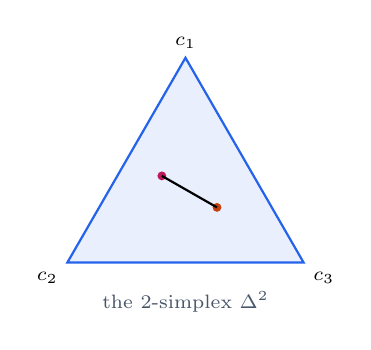
\begin{tikzpicture}[scale=1.0]
        \fill[cSimplex!10,draw=cSimplex,thick] (0,0)--(3,0)--(1.5,2.6)--cycle;
        \node[below left] at (0,0){\scriptsize $c_2$};
        \node[below right] at (3,0){\scriptsize $c_3$};
        \node[above] at (1.5,2.6){\scriptsize $c_1$};
        \fill[cAccent] (1.2,1.1) circle (1.6pt);
        \fill[cLik] (1.9,0.7) circle (1.6pt);
        \draw[thick] (1.2,1.1)--(1.9,0.7);
        \node[font=\scriptsize, cMuted] at (1.5,-0.5){the $2$-simplex $\Delta^{2}$};
      \end{tikzpicture}

      \vspace{0.6em}
      {\footnotesize Three model families, one taxonomy backbone:
      \textcolor{cSimplex}{\textbf{PhILR-VAE}} (isometry),
      \textcolor{cLik}{\textbf{TreeDTM-VAE}} (tree likelihood),
      \textcolor{cLatent}{\textbf{CAPDA-VAE}} (domain alignment).}
    \end{column}
  \end{columns}
\end{frame}

% ====================================================================
\section{PhILR-VAE}
% ====================================================================
\begin{frame}{PhILR-VAE --- a VAE in isometric log-ratio space}
  \textbf{Idea.} Map the simplex to flat space with a \emph{tree-defined isometry},
  run a vanilla Gaussian VAE there, and map back --- so Euclidean operations on the
  latent respect Aitchison geometry exactly.
  \begin{columns}[T]
    \begin{column}{0.46\textwidth}
      \textbf{Sequential Binary Partition (SBP).} Each internal node of the
      taxonomy splits its descendant leaves into $R$ ($|R|=r$) vs $S$ ($|S|=s$),
      giving one orthonormal \emph{balance}
      \[
        \psi_i=
        \begin{cases}
          +\sqrt{\dfrac{s}{r(r+s)}} & i\in R,\\[6pt]
          -\sqrt{\dfrac{r}{s(r+s)}} & i\in S,\\[2pt]
          0 & \text{otherwise.}
        \end{cases}
      \]
      Stacking $p-1$ balances gives $\Psi\in\R^{p\times(p-1)}$ with
      \[
        \langle\psi,\mathbf 1\rangle=0,\quad \Psi^\top\Psi=I_{p-1},
      \]
      spanning the clr-hyperplane $\mathbf 1^\perp$.
    \end{column}
    \begin{column}{0.54\textwidth}
      \centering
      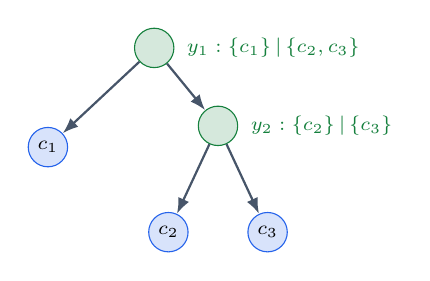
\begin{tikzpicture}[scale=0.9, every node/.style={font=\scriptsize}]
        \node[inode] (r) at (1.5,2.2){};
        \node[leaf]  (A) at (0,0.8){$c_1$};
        \node[inode] (m) at (2.4,1.1){};
        \node[leaf]  (B) at (1.7,-0.4){$c_2$};
        \node[leaf]  (C) at (3.1,-0.4){$c_3$};
        \draw[arrow] (r)--(A); \draw[arrow] (r)--(m);
        \draw[arrow] (m)--(B); \draw[arrow] (m)--(C);
        \node[cTree, right=1pt of r]{$y_1:\{c_1\}\,|\,\{c_2,c_3\}$};
        \node[cTree, right=1pt of m]{$y_2:\{c_2\}\,|\,\{c_3\}$};
      \end{tikzpicture}

      \vspace{0.4em}
      \begin{block}{Forward / inverse transform}
        \[
          \mathbf y=\ilr(\mathbf c)=\log(\mathbf c)\,\Psi\in\R^{p-1},\quad
          \hat{\mathbf c}=\softmax(\hat{\mathbf y}\,\Psi^\top).
        \]
      \end{block}
      \begin{exampleblock}{Isometry (Aitchison $\equiv$ Euclidean)}
        \[
          \big\|\mathbf y^{(1)}-\mathbf y^{(2)}\big\|_2
          = d_A\big(\mathbf c^{(1)},\mathbf c^{(2)}\big).
        \]
      \end{exampleblock}
    \end{column}
  \end{columns}
\end{frame}

\begin{frame}{PhILR-VAE --- computation graph}
  \centering
  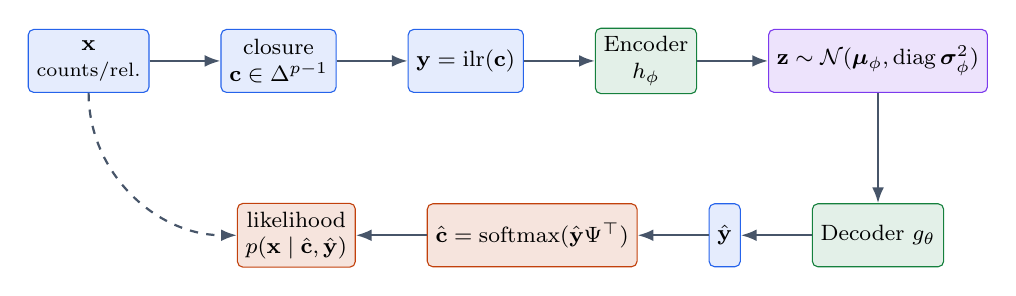
\begin{tikzpicture}[node distance=8mm and 9mm]
    \node[data] (x) {$\mathbf x$\\\scriptsize counts/rel.};
    \node[data, right=of x] (c) {closure\\$\mathbf c\in\Simplex$};
    \node[data, right=of c] (y) {$\mathbf y=\ilr(\mathbf c)$};
    \node[net,  right=of y] (enc) {Encoder\\$h_\phi$};
    \node[lat,  right=of enc] (z) {$\mathbf z\sim\mathcal N(\bm\mu_\phi,\diag\bm\sigma_\phi^2)$};
    \node[net,  below=14mm of z] (dec) {Decoder $g_\theta$};
    \node[data, left=of dec] (yh) {$\hat{\mathbf y}$};
    \node[lik,  left=of yh] (ch) {$\hat{\mathbf c}=\softmax(\hat{\mathbf y}\Psi^\top)$};
    \node[lik,  left=of ch] (lik) {likelihood\\$p(\mathbf x\mid\hat{\mathbf c},\hat{\mathbf y})$};
    \draw[arrow](x)--(c); \draw[arrow](c)--(y); \draw[arrow](y)--(enc);
    \draw[arrow](enc)--(z); \draw[arrow](z)--(dec); \draw[arrow](dec)--(yh);
    \draw[arrow](yh)--(ch); \draw[arrow](ch)--(lik);
    \draw[darrow](x.south) to[out=-90,in=180] (lik.west);
  \end{tikzpicture}

  \vspace{0.4em}
  \begin{columns}[T]
    \begin{column}{0.5\textwidth}
      \small
      \textbf{Encoder} $\mathbf x\!\to\!\mathbf c\!\to\!\mathbf y\!\to\!
      h_\phi(\mathbf y)\!\to\!(\bm\mu_\phi,\log\bm\sigma_\phi^2)$, with
      $\mathbf z=\bm\mu_\phi+\bm\sigma_\phi\odot\bm\varepsilon$.\\[2pt]
      \textbf{Decoder} $\mathbf z\to\hat{\mathbf y}\to
      \hat{\mathbf c}=\softmax(\hat{\mathbf y}\Psi^\top)\in\Simplex$
      (closure restored).
    \end{column}
    \begin{column}{0.5\textwidth}
      \begin{exampleblock}{Why principled}
        \footnotesize
        Outputs always lie in $\Simplex$; Euclidean decoding in ILR space is exact on
        the simplex, so \emph{no} extra geometric/consistency penalty is needed.
      \end{exampleblock}
    \end{column}
  \end{columns}
\end{frame}

\begin{frame}{PhILR-VAE --- likelihoods and objective}
  \begin{columns}[T]
    \begin{column}{0.6\textwidth}
      Five likelihoods share the encoder/decoder; only $\log p(\mathbf x)$ changes:
      \smallskip
      \begin{itemize}\small
        \item \textcolor{cLik}{\code{philr_gaussian}} (default, relative input) ---
              logistic-normal on $\Simplex$:
              $\;\mathbf y\sim\mathcal N(\hat{\mathbf y},\diag\bm\sigma_{\text{obs}}^2)$.
        \item \code{multinomial}: $\mathbf x\mid\hat{\mathbf c},N\sim
              \mathrm{Mult}(N,\hat{\mathbf c})$.
        \item \code{dirichlet_multinomial}: $\bm\alpha=\alpha_0\hat{\mathbf c}$,
              global overdispersion.
        \item \code{dirichlet_tree_multinomial}: per-clade DTM (shares the
              TreeDTM-VAE likelihood, next section).
        \item \code{dirichlet_tree}: continuous Dirichlet-tree for closed data.
      \end{itemize}
    \end{column}
    \begin{column}{0.4\textwidth}
      \begin{block}{ELBO objective}
        \[
          \mathcal L=-\,\E_{q_\phi}\!\big[\log p_\theta(\mathbf x\mid\mathbf z)\big]
          +\beta_t\,\KL\!\big(q_\phi\,\|\,\mathcal N(\mathbf 0,I)\big)
          +\gamma\,\mathcal R(\bm\theta_{\text{lik}})
        \]
        with closed-form Gaussian KL
        \[
          \KL=\tfrac12\sum_{j=1}^{d}\!\big(\mu_j^2+\sigma_j^2-1-\log\sigma_j^2\big),
        \]
        $\beta_t$ a linear warm-up, $\mathcal R$ a small $L_2$ on the
        likelihood parameters.
      \end{block}
    \end{column}
  \end{columns}
\end{frame}

% ====================================================================
\section{TreeDTM-VAE}
% ====================================================================
\begin{frame}{TreeDTM-VAE --- a likelihood at every internal node}
  \textbf{Idea.} Instead of a leaf-wise likelihood, factor the count distribution
  over the taxonomy: an independent \emph{local split} at every internal node, with
  overdispersion learned \emph{per clade}.
  \begin{columns}[T]
    \begin{column}{0.5\textwidth}
      \small
      Rooted tree $\Tree$ with internal nodes $\Inodes$, leaves $\mathcal L$.
      Observed vector $\mathbf y^{(i)}\in\R^{N}_{\ge 0}$ is aligned to \emph{every}
      node: leaves are raw counts, each internal entry is the sum of its children.
      \smallskip

      Decoder produces split logits, then a masked softmax per sibling group:
      \[
        \mathbf a^{(i)}=h_\theta(\mathbf z^{(i)})\in\R^{E},\;\;
        E=\!\!\sum_{u\in\Inodes}\!K_u,
      \]
      \[
        \pi^{(i)}_{u\to v}
        =\frac{\exp(a^{(i)}_{u\to v})}{\sum_{v'\in\Ch(u)}\exp(a^{(i)}_{u\to v'})},
        \quad v\in\Ch(u).
      \]
    \end{column}
    \begin{column}{0.5\textwidth}
      \centering
      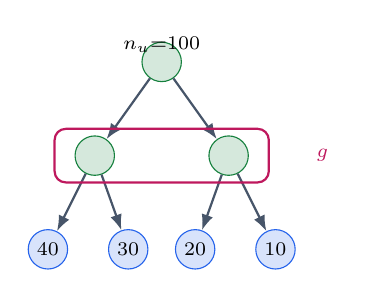
\begin{tikzpicture}[scale=0.85, every node/.style={font=\scriptsize}]
        \node[inode] (r) at (1.5,2.4){}; \node[above] at (r){$n_u{=}100$};
        \node[inode] (a) at (0.5,1.0){};
        \node[inode] (b) at (2.5,1.0){};
        \node[leaf] (l1) at (-0.2,-0.4){$40$};
        \node[leaf] (l2) at (1.0,-0.4){$30$};
        \node[leaf] (l3) at (2.0,-0.4){$20$};
        \node[leaf] (l4) at (3.2,-0.4){$10$};
        \draw[arrow] (r)--(a); \draw[arrow] (r)--(b);
        \draw[arrow] (a)--(l1); \draw[arrow] (a)--(l2);
        \draw[arrow] (b)--(l3); \draw[arrow] (b)--(l4);
        \draw[cAccent,thick,rounded corners] (-0.1,0.6) rectangle (3.1,1.4);
        \node[cAccent] at (3.9,1.0){$g$};
      \end{tikzpicture}

      \vspace{0.3em}
      \begin{block}{Sibling-centred log-ratio encoder}
        \footnotesize
        \[
          \ell^{(i)}_{u\to v}=\log(y^{(i)}_v+\tau)
          -\tfrac{1}{K_u}\!\!\sum_{v'\in\Ch(u)}\!\!\log(y^{(i)}_{v'}+\tau)
        \]
        gauge-fixes the within-group d.o.f.; MLP $g_\phi(\bm\ell)\to(\bm\mu_z,\log\bm\sigma_z^2)$.
      \end{block}
    \end{column}
  \end{columns}
\end{frame}

\begin{frame}{TreeDTM-VAE --- three node likelihoods}
  Joint log-likelihood is always a sum over internal nodes,
  $\log p(\mathbf y^{(i)}\mid\mathbf z^{(i)})=\sum_{u\in\Inodes}\log p(\mathbf x^{(i)}_u\mid\cdot)$,
  with child counts $\mathbf x^{(i)}_u=(x^{(i)}_{u\to v})_{v}$ and
  $n^{(i)}_u=\sum_v x^{(i)}_{u\to v}$.
  \begin{columns}[T]
    \begin{column}{0.5\textwidth}
      \begin{block}{Tree-Multinomial (no overdispersion)}
        \footnotesize
        \[
          p(\mathbf x_u\mid\bm\pi_{u})=
          \binom{n_u}{\mathbf x_u}\prod_{v\in\Ch(u)}\big(\pi_{u\to v}\big)^{x_{u\to v}}
        \]
      \end{block}
      \begin{alertblock}{Dirichlet-Tree-Multinomial (default)}
        \footnotesize
        Per-group concentration $\alpha^0_g>0$ from the decoder, $\bm\alpha^{(i)}_g=\alpha^0_g\,\bm\pi^{(i)}_g$:
        \[
          p(\mathbf x_u\mid\bm\alpha_g)=
          \binom{n_u}{\mathbf x_u}
          \frac{\Gamma(\alpha_{g,0})}{\Gamma(n_u+\alpha_{g,0})}
          \prod_v\frac{\Gamma(x_{u\to v}+\alpha_{g,v})}{\Gamma(\alpha_{g,v})}
        \]
        with $\alpha_{g,0}=\sum_v\alpha_{g,v}=\alpha^0_g$. Dispersion is
        \emph{per clade}.
      \end{alertblock}
    \end{column}
    \begin{column}{0.5\textwidth}
      \begin{block}{Continuous Dirichlet-Tree (closed data)}
        \footnotesize
        For $\mathbf c\in\Delta^{L-1}$, with child fractions
        $\mathbf q_u=\mathrm{normalise}(\mathbf x_u+\eta)$:
        \[
        \begin{aligned}
          \log p(\mathbf q_u\mid\bm\alpha_g)=&\;
          \log\Gamma(\alpha_{g,0})-\sum_v\log\Gamma(\alpha_{g,v})\\
          &+\sum_v(\alpha_{g,v}-1)\log q_{u\to v}.
        \end{aligned}
        \]
      \end{block}
      \begin{block}{Objective}
        \footnotesize
        \[
          \mathcal L^{(i)}=-\log p(\mathbf y^{(i)}\mid\mathbf z^{(i)})
          +\beta_t\,\KL\!\big(q_\phi\,\|\,\mathcal N(\mathbf 0,I)\big)
          +\gamma\,\|\bm\alpha^0\|^2,
        \]
        $\KL=\tfrac12\sum_j(\mu_{z,j}^2+\sigma_{z,j}^2-1-\log\sigma_{z,j}^2)$, optional
        free-bits floor.
      \end{block}
    \end{column}
  \end{columns}
\end{frame}

\begin{frame}{TreeDTM-VAE --- computation graph}
  \centering
  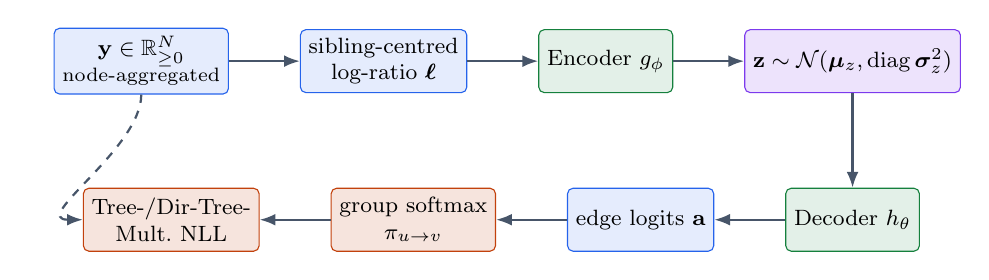
\begin{tikzpicture}[node distance=7mm and 9mm]
    \node[data] (y) {$\mathbf y\in\R^{N}_{\ge0}$\\\scriptsize node-aggregated};
    \node[data, right=of y] (l) {sibling-centred\\log-ratio $\bm\ell$};
    \node[net,  right=of l] (enc) {Encoder $g_\phi$};
    \node[lat,  right=of enc] (z) {$\mathbf z\sim\mathcal N(\bm\mu_z,\diag\bm\sigma_z^2)$};
    \node[net,  below=12mm of z] (dec) {Decoder $h_\theta$};
    \node[data, left=of dec] (a) {edge logits $\mathbf a$};
    \node[lik,  left=of a] (pi) {group softmax\\$\pi_{u\to v}$};
    \node[lik,  left=of pi] (nll) {Tree-/Dir-Tree-\\Mult.\ NLL};
    \draw[arrow](y)--(l);\draw[arrow](l)--(enc);\draw[arrow](enc)--(z);
    \draw[arrow](z)--(dec);\draw[arrow](dec)--(a);\draw[arrow](a)--(pi);\draw[arrow](pi)--(nll);
    \draw[darrow](y.south) to[out=-90,in=180] (nll.west);
  \end{tikzpicture}

  \vspace{0.3em}
  {\footnotesize Closure is enforced \emph{by the likelihood} (each sibling group
  is a proper multinomial / Dirichlet-multinomial), so proportions live exactly on
  the simplex --- statistically valid for both fixed-depth counts and pre-closed
  relative abundances.}
\end{frame}

% ====================================================================
\section{CAPDA-VAE}
% ====================================================================
\begin{frame}{CAPDA-VAE --- class-conditional, adversary-free domain alignment}
  \textbf{Idea.} A supervised, taxonomy-biased VAE that removes \emph{study} nuisance
  from $P(\mathbf z\mid y)$ \emph{without} an adversary, by pulling together same-class
  latent statistics across studies --- preserving the between-class signal that
  marginal DA-VAEs destroy under label shift.
  \begin{columns}[T]
    \begin{column}{0.52\textwidth}
      \begin{block}{Multi-resolution taxonomy input}
        \footnotesize
        Per-species CLR \emph{plus} abundances aggregated up the taxonomy
        (genus/family/order/phylum):
        \[
          \mathbf x=\big[\;\underbrace{\clr(\mathbf X)}_{\text{species}}
          \;\big|\;\underbrace{\log(1+\mathbf A_{g,f,o,p})}_{\text{aggregates}}\;\big],
        \]
        \[
          \clr(\mathbf X)_i=\log(X_i+\epsilon)-\tfrac1p\!\sum_j\log(X_j+\epsilon).
        \]
      \end{block}
      \begin{block}{Network}
        \footnotesize
        MLP encoder $\to(\bm\mu,\log\bm\sigma^2)$, $\mathbf z=\bm\mu+\bm\sigma\odot\bm\varepsilon$;
        MLP decoder $\to\hat{\mathbf x}$; \textbf{class head} on the latent
        $\bm\ell_{\text{cls}}=\mathrm{cls}(\mathbf z)$.
      \end{block}
    \end{column}
    \begin{column}{0.48\textwidth}
      \centering
      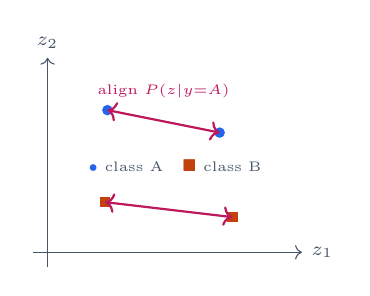
\begin{tikzpicture}[scale=0.95, every node/.style={font=\scriptsize}]
        \draw[->,cMuted] (-0.2,0)--(3.4,0); \draw[->,cMuted] (0,-0.2)--(0,2.6);
        \node[cMuted,right] at (3.4,0){$z_1$}; \node[cMuted,above] at (0,2.6){$z_2$};
        % class A (circles) two studies
        \fill[cSimplex] (0.8,1.9) circle (2pt);
        \fill[cSimplex] (2.3,1.6) circle (2pt);
        \draw[<->,cAccent,thick] (0.8,1.9)--(2.3,1.6);
        \node[cAccent] at (1.55,2.15){\tiny align $P(z|y{=}A)$};
        % class B (squares) two studies
        \fill[cLik] (0.7,0.6) rectangle (0.84,0.74);
        \fill[cLik] (2.4,0.4) rectangle (2.54,0.54);
        \draw[<->,cAccent,thick] (0.77,0.67)--(2.47,0.47);
        \node[cMuted] at (1.7,1.15){\tiny \textcolor{cSimplex}{$\bullet$} class A \;
          \textcolor{cLik}{$\blacksquare$} class B};
      \end{tikzpicture}

      {\footnotesize Same-class study means pulled to a shared per-class
      centroid; different classes stay apart.}
    \end{column}
  \end{columns}
\end{frame}

\begin{frame}{CAPDA-VAE --- conditional alignment (adversary-free)}
  For class $c$ and study $s$, let the per-(study,class) latent mean be
  $\mathbf m_{c,s}=\operatorname{mean}\{\bm\mu_i : y_i=c,\,d_i=s\}$ and the class
  centroid $\bar{\mathbf m}_c=\operatorname{mean}_s \mathbf m_{c,s}$ (over studies present).
  \begin{columns}[T]
    \begin{column}{0.5\textwidth}
      \begin{block}{First moment (conditional mean)}
        \[
          \mathcal A_{1}=\frac{1}{|\mathcal C'|}\sum_{c\in\mathcal C'}
          \frac{1}{|\mathcal S_c|}\sum_{s\in\mathcal S_c}
          \big\|\mathbf m_{c,s}-\bar{\mathbf m}_c\big\|_2^2 ,
        \]
        over classes $\mathcal C'$ seen in $\ge 2$ studies.
      \end{block}
      \begin{block}{Second moment (conditional CORAL)}
        \[
          \mathcal A_{\mathrm{cov}}=\frac{1}{|\mathcal C''|}\sum_{c\in\mathcal C''}
          \sum_{s}\big\|\Cov_{c,s}-\bar{\bm\Sigma}_c\big\|_F^2,
        \]
        with $\Cov_{c,s}=\Cov(\bm\mu : y{=}c,d{=}s)$,
        $\bar{\bm\Sigma}_c=\operatorname{mean}_s\Cov_{c,s}$.
      \end{block}
    \end{column}
    \begin{column}{0.5\textwidth}
      \begin{alertblock}{Total objective}
        \[
        \begin{aligned}
          \mathcal L=\;&\underbrace{\|\hat{\mathbf x}-\mathbf x\|_2^2}_{\text{recon (MSE)}}
          +\beta_t\,\KL +\alpha\,\CE(\bm\ell_{\text{cls}},y;\,\mathbf w)\\
          &+\lambda_t\,\mathcal A_{1}
          +\frac{\lambda_t}{\gamma}\,\gamma_{\mathrm{cov}}\,\mathcal A_{\mathrm{cov}},
        \end{aligned}
        \]
        $\CE$ class-weighted; $\beta_t,\lambda_t$ linear warm-ups
        ($\lambda_t=\gamma\min(1,\,t/T_{\text{align}})$).
      \end{alertblock}
    \end{column}
  \end{columns}
\end{frame}

\begin{frame}{CAPDA-VAE --- why \emph{conditional}? the taxonomy/invariance trade-off}
  \begin{columns}[T]
    \begin{column}{0.58\textwidth}
      A formal trade-off governs taxonomy bias vs.\ domain invariance on the
      balanced two-study risk $\mathcal E$:
      \begin{block}{Taxonomy upper bound (T)}
        \footnotesize
        A taxonomy-aware backbone (PhILR / TreeDTM) with no invariance constraint
        attains
        $\;\mathcal E_{\text{(T)}}\le \widehat{\mathcal E}+\mathcal O\!\big(\sqrt{\mathfrak C(\mathcal F_\Tree)/n}\big)$,
        the variance-reduction half.
      \end{block}
      \begin{alertblock}{Invariance lower bound (I)}
        \footnotesize
        Enforcing \emph{marginal} domain invariance (DIVA / PhyloDIVA style) costs
        $\;\mathcal E_{\text{(I)}}\ge \tfrac{\Delta_Y}{2}-\delta$,
        where $\Delta_Y$ is the between-study label shift. Invariance \emph{hurts}
        precisely when composition shifts with the label.
      \end{alertblock}
    \end{column}
    \begin{column}{0.42\textwidth}
      \begin{exampleblock}{CAPDA's resolution}
        \footnotesize
        Align \emph{within each class} ($P(\mathbf z\mid y)$), not the marginal
        $P(\mathbf z)$. This removes the study nuisance term without paying the
        $\Delta_Y/2$ penalty of (I) --- and keeps the taxonomy bias (T) via the
        multi-resolution CLR input. Adversary-free: alignment is a closed-form
        moment-matching penalty, not a min-max game.
      \end{exampleblock}
      \begin{block}{Single-study limit}
        \footnotesize
        With one domain, $\mathcal A_1\!=\!\mathcal A_{\mathrm{cov}}\!\equiv\!0$ (any class
        needs $\ge2$ studies): CAPDA degrades gracefully to a supervised taxonomy-biased
        VAE with leak-free stratified $K$-fold OOF stacking.
      \end{block}
    \end{column}
  \end{columns}
\end{frame}

% ====================================================================
\section*{Summary}
% ====================================================================
\begin{frame}{Summary --- three compositional VAEs}
  \small
  \renewcommand{\arraystretch}{1.35}
  \begin{tabular}{@{}L{2.0cm}L{3.5cm}L{3.4cm}L{3.4cm}@{}}
    \toprule
     & \textcolor{cSimplex}{\textbf{PhILR-VAE}}
     & \textcolor{cLik}{\textbf{TreeDTM-VAE}}
     & \textcolor{cLatent}{\textbf{CAPDA-VAE}}\\
    \midrule
    Encoder input & ILR coords $\mathbf y=\log(\mathbf c)\Psi$
                  & sibling-centred log-ratios per node
                  & $[\clr(\text{species})\mid\log\text{-agg}]$\\
    Tree enters via & SBP contrast basis $\Psi$
                    & per-node likelihood factorisation
                    & multi-resolution aggregation\\
    Likelihood & logistic-normal / multinomial / DTM
               & Tree-/Dir-Tree-Multinomial
               & Gaussian recon + class head\\
    Extra term & --- (isometry is exact)
               & per-clade $\|\bm\alpha^0\|^2$
               & conditional align $\mathcal A_1,\mathcal A_{\mathrm{cov}}$\\
    Best for & metric / embedding quality
             & clade-specific overdispersion
             & cross-cohort label prediction\\
    \bottomrule
  \end{tabular}
  \vfill
  {\footnotesize All three: standard Gaussian latent $\mathcal N(\mathbf 0,I)$,
  reparameterised sampling, ELBO with linear $\beta_t$ warm-up.
  Theory: \code{docs/philrvae_theory.md}, \code{docs/tree_dtm_vae_theory.md},
  \code{docs/capda_vae_theory.md}.}
\end{frame}

\end{document}
